\subsection{Tensorflow}
\index{Tensorflow}

% Introduction {{{
\begin{figure}[H]
  \centering
  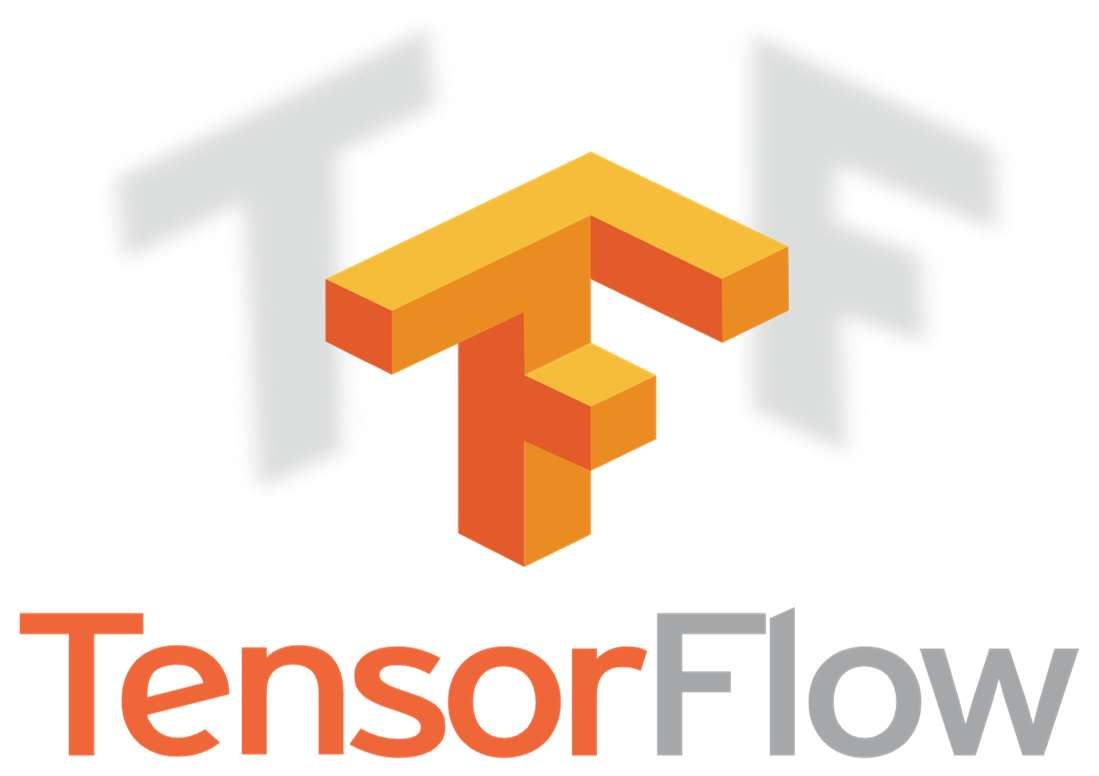
\includegraphics[width=\linewidth/2]{%
    diagrams/tensorflow_logo.png}
  \caption{Tensorflow Logo}
\end{figure}

Tensorflow is a powerful data flow-oriented machine
learning library created Google's Brain Team and made open
source in 2015. It is designed to be easy to use and widely
applicable to both numeric and neural network-oriented
problems as well as other domains.\cite{david3}

It uses Python to provide a convenient front-end API for
building applications with this framework, while executing
those applications in a high-performance C++ environment.

Tensorflow can train and run deep neural networks making it
possible to write models for a variety of different tasks,
including handwritten digit classification, image
recognition, word embeddings, recurrent neural networks,
sequence-to-sequence models for machine translation,
natural language processing or PDE (partial differential
equation) based simulations. Best of all, Tensorflow
supports production prediction at scale, with the same
models used for training.\cite{david5}
% }}}

% History {{{
\subsubsection{History}

Starting in 2011, Google Brain built DistBelief as a
proprietary machine learning system based on deep learning
neural networks. Its use grew rapidly across diverse
Alphabet companies in both research and commercial
applications. Google assigned multiple computer scientists,
including Jeff Dean, to simplify and refactor the codebase
of DistBelief into a faster, more robust application-grade
library.\cite{david7}

The source code of DistBelief was modified and made into a
much better application-based library and soon in 2015 came
to be known as Tensorflow. Tensorflow is Google Brain's
second-generation system. Version 1.0.0 was released on
February 11, 2017.\cite{david3} The latest release of
Tensorflow is 1.9.0. It was released on 10.07.2018 and is
available at \url{www.tensorflow.org}.
% }}}

% How Tensorflow works {{{
\subsubsection{How Tensorflow works}

Tensorflow is cross-platform. It runs on nearly everything:
GPUs and CPUs—including mobile and embedded platforms—and
even tensor processing units (TPUs), which are specialized
hardware to do tensor math on.\cite{david1}

The easiest way to understand Tensorflow and Google's
approach to AI is with image recognition. In 2011, Google
created DistBelief, which used machine learning to identify
what's in a photo by recognizing certain patterns. For
example, it will look for whiskers of a certain length to
help determine if the image is of a cat.

The system was built using positive reinforcement —
essentially, the machine was given an image and asked if
the image was a cat. If the machine was correct, it was
told so. But if the machine was wrong, the system was
adjusted to recognize different patterns in an image so
that it was more likely to get it right next time.

Tensorflow takes the concept a step further by using deep
learning, or an artificial neural network composed of many
layers.

Basically, Tensorflow sorts through layers of data, called
nodes, to learn that the image it is viewing is of a cat.
The first layer will ask the system to look for something
as basic as determining the general shape in the picture.
The system then moves, or flows, to the next data set —
like looking for paws in the photo.\cite{david6}
\index{Tensorflow!nodes}

Tensorflow allows developers to create dataflow graph—
structures that describe how data moves through a graph, or
a series of processing nodes. Each node in the graph
represents a mathematical operation, and each connection or
edge between nodes is a multidimensional data array, or
tensor.

Tensorflow provides all of this for the programmer by way
of the Python programming language (cmp. \ref{s_python}).
Python is easy to learn and work with and provides
convenient ways to express how high-level abstractions can
be coupled together. Nodes and tensors in Tensorflow are
Python objects and Tensorflow applications are themselves
Python applications.

The actual math operations, however, are not performed
using Python. The libraries of transformations that are
available through Tensorflow are written as
high-performance C++ binaries. Python just directs traffic
between the pieces and provides high-level programming
abstractions to hook everyting together.

Tensorflow applications can be run on mostly any target
that’s convenient: a local machine, a cluster in the cloud,
iOS and Android devices, CPUs or GPUs. If you use Google’s
own cloud solution, you can run Tensorflow on Google’s
custom Tensorflow Processing Unit (TPU) for further
acceleration. The resulting models created by Tensorflow,
though, can be deployed on most any device where they will
be used to serve predictions.\cite{david5}

\newpage

\begin{figure}[H]
  \centering
  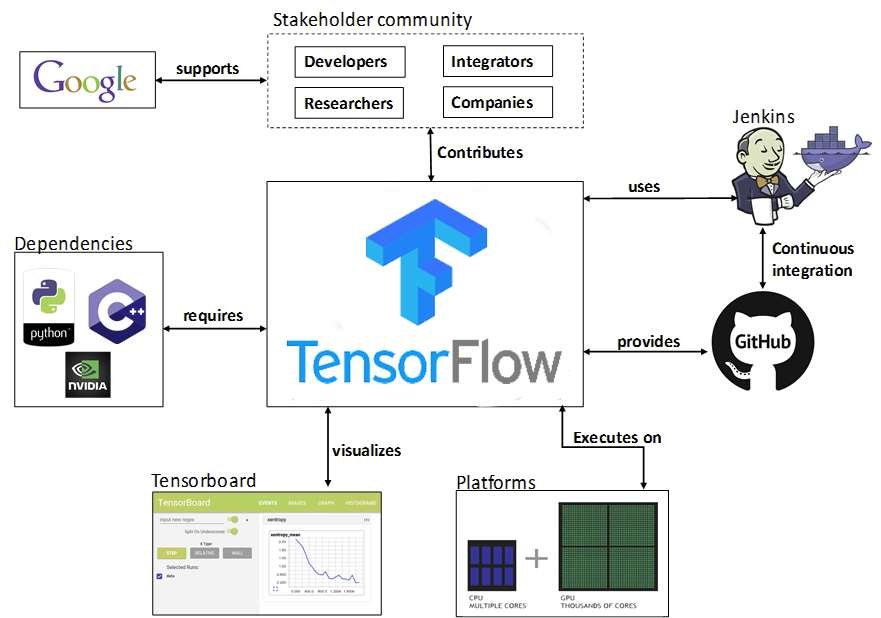
\includegraphics[width=\linewidth]{%
    diagrams/tensorflow_ecosys.png}
  \caption{Scheme of the Tensorflow Ecosystem\cite{david3}}
\end{figure}
% }}}

% Computational Optimizations {{{
\subsubsection{Computational Optimizations}

While Tensorflow uses every resource of a system available
(CPUs, GPUs, etc.) it also tries to optimize computation
havy tasks which includes machine learning to the fullest.
In our apllication our agent is running on Tensorflow so
training and predicting can be done fast and concurrent.

Some ways Tensorflow optimzes computation heavy tasks:

\begin{itemize}[label={}]

  \item \textbf{Common Fused Ops:}

        These operations merge more than one operation
        into a single kernel to improve the performance.
        XLA (Accelerated Linear Algebra - Optimzer for
        Tensorflow computations) creates these operations
        whenever possible to improve performance
        automatically.

  \item \textbf{Fused Batch Normalization:}

        An expensive process in TensorFlow performance
        optimization with a large amount of operation time.
        We use it to combine several operations into a
        single kernel to perform the batch normalization.
        Using this can speed up the process up to 12-30\%.
        \cite{david3}


  \item \textbf{Optimizing for GPU:}

        Optimal performance with the GPU seems to be the
        ultimate aim and one of the ways of achieving this
        is with the use of parallelism.
        Parallelism/concurrency is optainable by making
        multiple copies of the model (a neural network)
        that are refered to as towers.

        A tower is placed on each of the GPUs. The towers
        work on different batches of data (for training or
        predicting), updating variables (parameters) of
        the neural network which are shared between each
        tower (only training).

        Updates of these parameters depend upon the model
        and the configuration of the hardware.

  \item \textbf{Optimizing for CPU:}

        Tensorflow can optimize its computations for a CPU,
        as long as Tensorflow's whole instruction set is
        supported (which basically excludes older CPUs,
        like we used in our development environment).

        Tensorflow works with thread pools for optimizing
        the computations with concurrency.

        Now, to optimize the thread pools (the amount of
        threads which are used, based on the CPUs of the
        system), Tensorflow has two pools which sizes
        can be set with configuration parameters which can
        be changed by the developer\cite{tf_op}:

        \begin{itemize}

          \item \textbf{intra\_op\_parallelism:}

                Nodes which can compute concurrently
                schedule their parts into this thread pool.
                Changeing this value will change the amount
                of threads used.\cite{tf_op}

          \item \textbf{inter\_op\_parallelism:}

                The nodes that are ready are scheduled in
                this thread pool.\cite{tf_op}

        \end{itemize}

        For both, default configuration is zero,
        which forces Tensorflow to take the amount of
        available logical cores as the amount of threads
        for both pools.

        "Testing has shown that the default is effective
        for systems ranging from one CPU with 4 cores to
        multiple CPUs with 70+ combined logical cores".
        \cite{tf_op}

\end{itemize}


% }}}
